\chapter{Other appendixes}
\label{annexe:five}

\fancyhead[LE]{\textsc{\chaptername~\thechapter}}

\section{Cheaters in CS2}

Community-driven data aggregation suggests that the actual prevalence of cheaters in CS2 matchmaking is lower than subjective perception implies — Figure 7 shows one such analysis, estimating a 6.6\% chance of a cheater being present in a given game across approximately 3,000 matches at an average elo of 6,900.

\begin{figure}[h]
    \begin{center}
        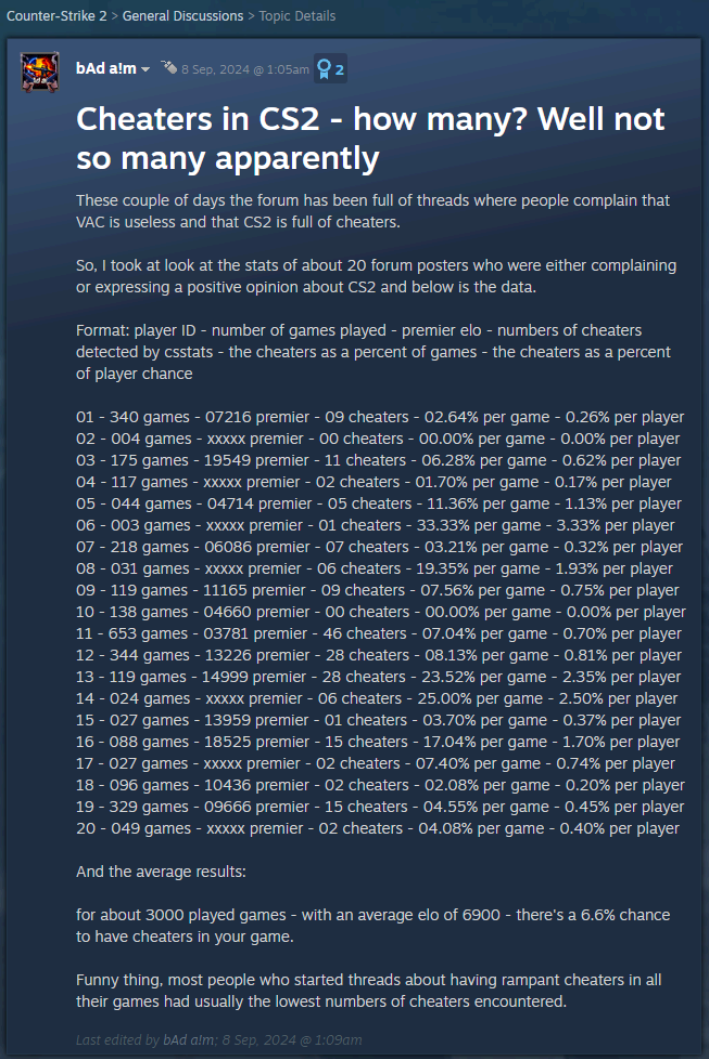
\includegraphics[height=19cm]{../images/annex05/cheaters.png}
    \end{center}
    \caption[Data aggregation made by a CS2 player to show the chance of a cheater being in a game.]{https://steamcommunity.com/app/730/discussions/0/4753074843849422337/}
    \label{fig:cheaters}
\end{figure}

\section{Existing data aggregation tool}

Third-party platforms already aggregate match telemetry into rich per-player behavioral profiles, as shown in Figure 8, demonstrating that demo-derived data is sufficiently granular to serve as a foundation for the suspicion-scoring pipeline developed in Chapter 3.

\begin{figure}[h]
    \begin{center}
        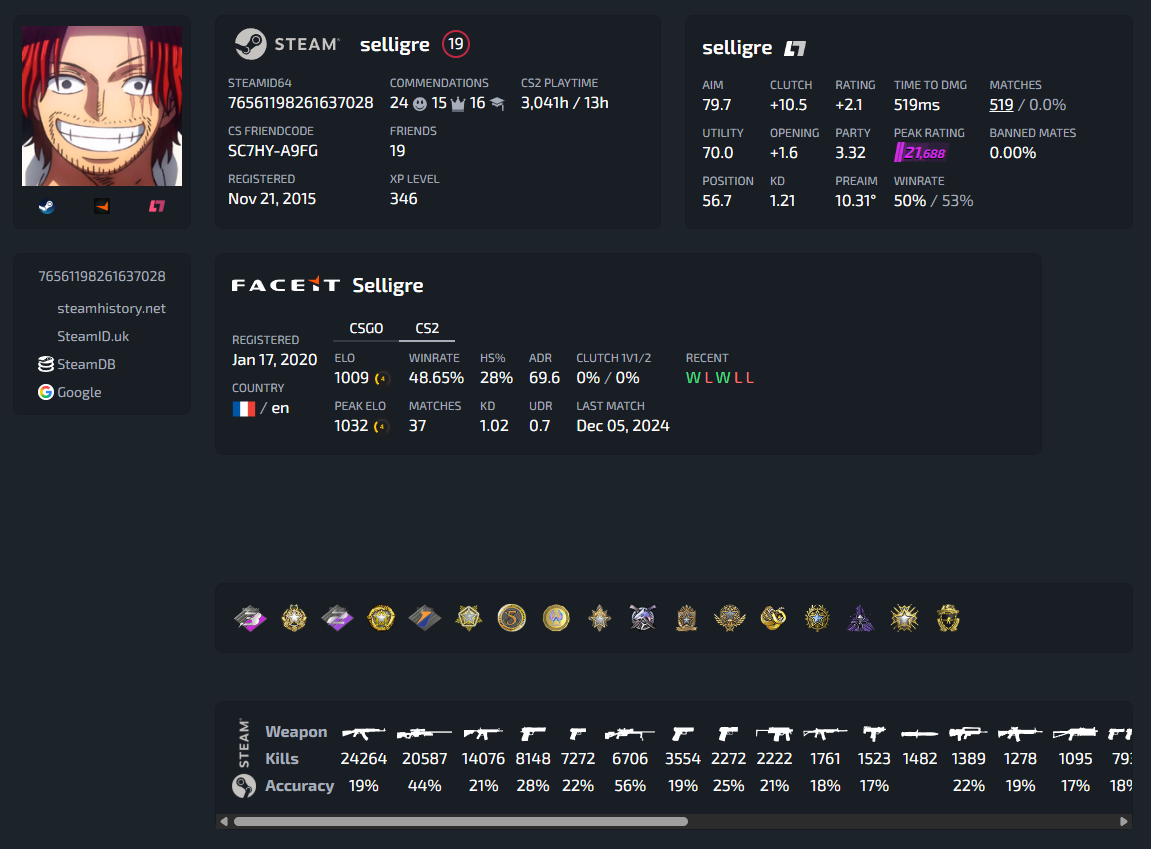
\includegraphics[height=11cm]{../images/annex05/csst.png}
    \end{center}
    \caption[Existing data aggregation tool to help visualize a player's game statistics.]{https://csst.at/profile/76561198261637028}
    \label{fig:csst}
\end{figure}
